\documentclass[11pt]{article}
\usepackage[margin=1in]{geometry}
\usepackage{amsmath,amssymb}
\usepackage{booktabs}
\usepackage{graphicx}
\usepackage{caption}
\usepackage{subcaption}
\usepackage{float}
\usepackage[authoryear,round]{natbib}
\usepackage{hyperref}
\hypersetup{pdfauthor={Qiaoshi Yang},
  pdftitle={Did Massachusetts' 1992 Tobacco Control Initiative Reduce Cigarette Sales?},
  colorlinks=true, linkcolor=black, citecolor=black, urlcolor=blue}
\graphicspath{{../output/}}
\setlength{\parskip}{0.4em}

\title{Did Massachusetts' 1992 Tobacco Control Initiative Reduce Cigarette Sales?\\
  \large Evidence from Synthetic Control and Synthetic Difference-in-Differences}
\author{Qiaoshi Yang\\ STAT 5200: Applied Econometrics, Final Project}
\date{\today}

\begin{document}
\maketitle

\begin{abstract}
In November 1992 Massachusetts voters approved Question~1, which raised the
cigarette excise tax by 25 cents per pack and used the revenue to fund a
statewide tobacco control program. I estimate its effect on per-capita
cigarette sales with the synthetic control method of \citet{adh2010}, after
first replicating their estimate for California's Proposition~99 with the same
code. Synthetic Massachusetts, a weighted average of Connecticut, Delaware, Utah
and Rhode Island, tracks Massachusetts closely from 1970 to 1992. After 1992
the two diverge: by 2000 actual sales are 29 packs per capita below the
synthetic counterfactual, and the average gap over 1993--2000 is 18.5 packs, or
21\% of counterfactual sales. Massachusetts has the third-largest post/pre fit
ratio among 39 states (permutation $p = 0.077$) and the largest standardised
reduction ($p = 0.026$). Two-way fixed effects DiD and synthetic DiD give
average effects of $-19$ and $-17$ packs. Single-treated-unit uncertainty is
large, though: synthetic DiD's placebo standard error is 11 packs.
Code and data: \url{https://github.com/yang-qs/stat5200-project}.
\end{abstract}

%======================================================================
\section{Introduction}

Between 1988 and 1992 two U.S.\ states passed ballot initiatives that combined
a cigarette tax increase with an earmarked anti-smoking program. California's
Proposition~99 (1988) raised the tax by 25 cents and funded media campaigns,
school programs and local coalitions. Four years later Massachusetts' Question~1
did nearly the same thing: the tax rose from 26 to 51 cents per pack on
1~January 1993, and the revenue financed the Massachusetts Tobacco Control
Program (MTCP). Whether such programs reduce smoking beyond what the tax alone
would do is a recurring question in tobacco policy, and these two states are its
standard test cases.

California's program is the canonical application of the synthetic control
method. \citet{adh2010} build a ``synthetic California'' from 38 states without
large tobacco programs and find that by 2000 per-capita sales were about 26
packs lower than they would have been without Proposition~99. Earlier
evaluations of Massachusetts used simpler comparisons. \citet{harris1996}
compare Massachusetts with the other 48 contiguous states and report a faster
decline in sales after 1992, and \citet{biener2000} report similar trends using
sales and survey data. Neither builds a counterfactual from pre-treatment data
or quantifies uncertainty for a single treated state.

This project adds two things. First, it asks whether the California result
generalises to the only other state that adopted a comparable program in that
period, using the same data, donor pool and estimator, so that differences in
the answer are not artefacts of method. Second, it puts the synthetic control
estimate next to two-way fixed effects DiD and the synthetic DiD estimator of
\citet{arkhangelsky2021}. This shows how much the conclusion depends on the
choice between DiD-type and SC-type estimators, and how wide honest
single-unit confidence bands are. A by-product is an estimate of how much of the
decline can plausibly be explained by the price increase alone.

%======================================================================
\section{Data}

\paragraph{Outcome and prices.}
The main source is \emph{The Tax Burden on Tobacco, 1970--2019}
\citep{orzechowski2019}, distributed by the CDC STATE System. It reports, for
each state and fiscal year (ending 30 June), per-capita cigarette pack sales
(computed from tax-paid sales), the average retail price per pack and the state
and federal excise taxes. \citet{adh2010} use the same series. Because the
data are by fiscal year, the January 1993 tax increase falls in the middle of
fiscal 1993; following the convention \citet{adh2010} use for California's
January 1989 increase, fiscal 1993 is the first treated year, and Section~4.4
shows that using 1994 instead changes nothing. The sample is 1970--2000: 23
pre-treatment and 8 post-treatment years for Massachusetts.

\paragraph{Covariates.}
To reproduce the predictors of \citet{adh2010} I merge three further
state-year series: per capita personal income from the BEA (table SAINC1,
logged); the share of the population aged 15--24, built from NCI SEER county
population estimates; and beer consumption in gallons per resident aged 14 and
over, from the NIAAA apparent-consumption file. Income is in nominal dollars.
Since every state's predictors are averaged over the same years, a common price
deflator cancels out of the comparison.

\paragraph{Donor pool.}
I use the donor pool of \citet{adh2010}: all states except those that adopted
large tobacco control programs (Arizona, California, Florida, Massachusetts and
Oregon), those that raised cigarette taxes by 50 cents or more between 1989 and
2000 (Alaska, Hawaii, Maryland, Michigan, New Jersey, New York and Washington),
and the District of Columbia. This leaves 38 donor states.

Table~\ref{tab:desc} and Figure~\ref{fig:trends} describe the data. Before 1993
Massachusetts sold about 11 packs per capita fewer than the average donor, and
its sales were falling faster than the donor average during the late 1980s.
That pre-trend is the main reason a simple comparison of means is not enough.
The naive difference in mean changes is $-19.3$ packs.

\begin{table}[H]\centering\small
\caption{Means (standard deviations) over state-years.}\label{tab:desc}
\begin{tabular}{lcccc}
\toprule
 & \multicolumn{2}{c}{Massachusetts} & \multicolumn{2}{c}{Donor pool (38 states)} \\
\cmidrule(lr){2-3}\cmidrule(lr){4-5}
 & 1970--92 & 1993--2000 & 1970--92 & 1993--2000 \\
\midrule
Packs per capita & 115.56 (9.65) & 70.20 (9.24) & 126.23 (32.53) & 100.20 (24.01) \\
Retail price (\$/pack) & 0.94 (0.46) & 2.66 (0.71) & 0.85 (0.44) & 2.07 (0.54) \\
State tax (\$/pack) & 0.21 (0.04) & 0.57 (0.18) & 0.14 (0.07) & 0.26 (0.14) \\
Tax share of price (\%) & 39.85 (9.43) & 35.49 (4.67) & 34.61 (9.67) & 26.03 (6.54) \\
\bottomrule
\end{tabular}

\par\smallskip\footnotesize Tax share is federal plus state tax as a share of
the retail price, recomputed from its components.
\end{table}

\begin{figure}[H]\centering
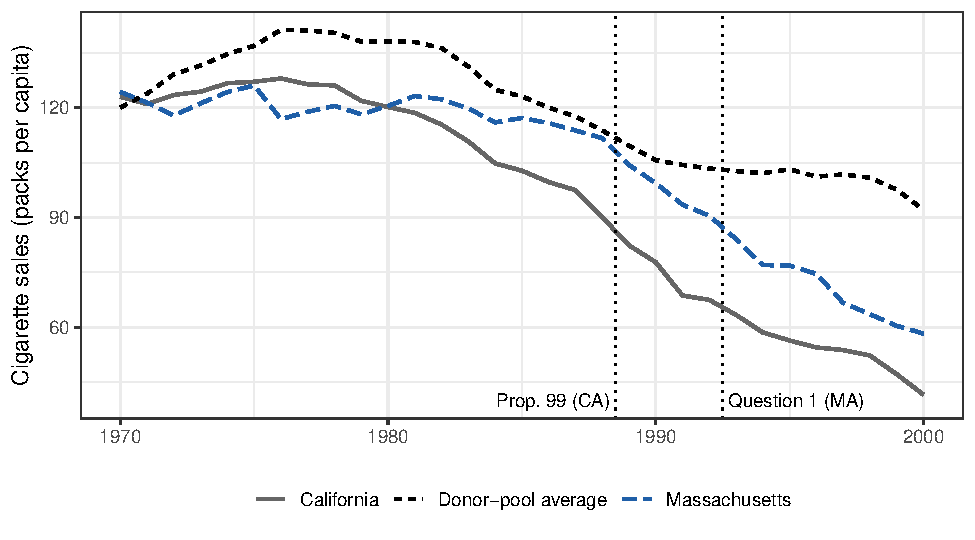
\includegraphics[width=0.8\textwidth]{trends.pdf}
\caption{Per-capita cigarette sales, 1970--2000. Dotted lines mark the first
treated years for California (1989) and Massachusetts (1993).}\label{fig:trends}
\end{figure}

%======================================================================
\section{Models}

Index states by $j = 1,\dots,J+1$, with $j=1$ the treated state and
$j = 2,\dots,J+1$ the $J = 38$ donors, and years by $t = 1,\dots,T$, with
$T_0$ the last untreated year. Let $Y_{jt}^N$ be per-capita sales without the
program and $Y_{jt}^I$ sales with it. The parameters of interest are the yearly
effects $\alpha_{1t} = Y_{1t}^I - Y_{1t}^N$ for $t > T_0$ and their average
$\bar\alpha = (T-T_0)^{-1}\sum_{t>T_0}\alpha_{1t}$. Only $Y_{1t}^I$ is observed
after $T_0$, so each method is a way of imputing $Y_{1t}^N$.

\subsection{Synthetic control}
The synthetic control estimator \citep{abadie2003, adh2010} imputes
$\hat Y_{1t}^N = \sum_{j\ge 2} w_j Y_{jt}$ with weights $w_j \ge 0$,
$\sum_j w_j = 1$. Given a $k\times 1$ vector of pre-treatment predictors
$X_1$ for the treated state and the matrix $X_0$ for donors, the weights solve
\begin{equation}
  W^*(V) = \arg\min_{W}\; (X_1 - X_0W)'V(X_1 - X_0W),
\end{equation}
and the diagonal matrix $V$ is chosen to minimise the pre-treatment mean
squared prediction error (MSPE) of the outcome. Following \citet{adh2010}, the
predictors are the averages of log income, retail price and the 15--24
population share over the nine years before treatment, average beer
consumption over the five years before treatment, and per-capita sales in 1975,
1980 and the last pre-treatment year (1988 for California, 1992 for
Massachusetts). The estimator is implemented with the \texttt{Synth} R package.

Inference uses placebos in space. Each donor in turn is treated as if it had
adopted the program, with the other 38 states as its donor pool, and the
ratio of post- to pre-treatment root MSPE is computed for each of the 39
units. The permutation $p$-value is the treated state's rank on this ratio
divided by 39. Because the ratio uses squared gaps, it is two-sided and treats a
large increase like a large decrease. I also report a one-sided version that
ranks the signed statistic $\bar\alpha_j/\mathrm{RMSPE}_j^{\text{pre}}$.

\subsection{Two-way fixed effects DiD}
The DiD benchmark is
\begin{equation}
  Y_{jt} = \mu_j + \lambda_t + \tau\, D_{jt} + \varepsilon_{jt},
  \qquad D_{jt} = \mathbf 1\{j = 1,\ t > T_0\},
\end{equation}
estimated on the treated state and the 38 donors, which weights all donors
equally and assumes parallel trends. With a single treated state,
cluster-robust standard errors are not valid \citep{conley2011}, so I report
them only for reference and base inference on the same placebo-in-space
permutation as for the synthetic control. I also estimate an event-study
version with separate coefficients for each year relative to 1993, to see
whether the parallel-trends assumption is plausible before 1993.

\subsection{Synthetic difference-in-differences}
Synthetic DiD \citep{arkhangelsky2021} combines the two:
\begin{equation}
  (\hat\tau, \hat\mu, \hat\alpha, \hat\beta) = \arg\min
  \sum_{j}\sum_{t} \bigl(Y_{jt} - \mu - \alpha_j - \beta_t - \tau D_{jt}\bigr)^2
  \hat\omega_j \hat\lambda_t,
\end{equation}
where unit weights $\hat\omega$ make the weighted donor trend match the treated
state's pre-treatment trend (not its level, because unit fixed effects remain)
and time weights $\hat\lambda$ put weight on the pre-treatment years most
similar to the post-treatment period. With $\hat\omega_j = 1/J$ and uniform
$\hat\lambda$ the estimator is the DiD above. Without fixed effects it is a
synthetic control using only outcomes. I estimate all three variants with the
\texttt{synthdid} package and use its placebo variance estimator, the only one
available with one treated unit.

\subsection{Implied price response}
Estimating the DiD model with $\log Y_{jt}$ and with the log retail price as
outcomes gives the program's effect on log sales, $\tau_q$, and on log price,
$\tau_p$. The ratio $\tau_q/\tau_p$ is a Wald estimate of the price elasticity
of demand, but only if the program affects sales through the price. Comparing it
with elasticities from the literature indicates how much of the decline the tax
alone can account for.

%======================================================================
\section{Results}
All code is in the GitHub repository
\url{https://github.com/yang-qs/stat5200-project}. \texttt{Rscript run\_all.R}
downloads the raw data and regenerates every number, table and figure in this
report, and the README lists what each script does.

\subsection{Replication: California}\label{sec:repl}
The replication reproduces the main results of \citet{adh2010}. Synthetic
California is a combination of Utah (0.37), Colorado (0.32), Nevada (0.24) and
Connecticut (0.08); ADH report Utah, Nevada, Montana, Colorado and Connecticut.
The predictors are well balanced (Table~\ref{tab:bal}, left), and the
pre-treatment RMSPE is 1.95 packs. The estimated gap in 2000 is $-24.3$ packs
per capita, compared with about $-26$ in the paper, and California has the
largest post/pre RMSPE ratio of the 39 states, so the permutation $p$-value is
$1/39 = 0.026$, as in the original. The small differences in weights and in
the size of the gap are plausibly due to revisions of the tobacco series since
2010 and to my covariates being rebuilt from current releases of the BEA, SEER
and NIAAA files. Figure~\ref{fig:ca} in the appendix shows the paths.

\begin{table}[H]\centering\small
\caption{Predictor balance: treated state, synthetic control and donor average.}\label{tab:bal}
\begin{subtable}{0.49\textwidth}\centering\resizebox{\linewidth}{!}{\begin{tabular}{lccc}
\toprule
 & California & Synthetic & Donor average \\
\midrule
Ln(per capita income) & 9.65 & 9.49 & 9.42 \\
Retail price (\$/pack) & 0.97 & 0.98 & 0.95 \\
Share aged 15--24 (\%) & 17.32 & 17.04 & 17.30 \\
Beer per capita (gal.) & 29.79 & 30.03 & 30.27 \\
Packs per capita, 1975 & 127.10 & 126.73 & 136.93 \\
Packs per capita, 1980 & 120.20 & 120.44 & 138.09 \\
Packs per capita, 1988 & 90.10 & 92.11 & 113.82 \\
\bottomrule
\end{tabular}
}
\caption{California (1989)}\end{subtable}\hfill
\begin{subtable}{0.49\textwidth}\centering\resizebox{\linewidth}{!}{\begin{tabular}{lccc}
\toprule
 & Massachusetts & Synthetic & Donor average \\
\midrule
Ln(per capita income) & 9.92 & 9.88 & 9.66 \\
Retail price (\$/pack) & 1.44 & 1.44 & 1.32 \\
Share aged 15--24 (\%) & 16.30 & 15.85 & 15.67 \\
Beer per capita (gal.) & 26.83 & 25.54 & 29.86 \\
Packs per capita, 1975 & 126.10 & 119.03 & 136.93 \\
Packs per capita, 1980 & 120.50 & 123.18 & 138.09 \\
Packs per capita, 1992 & 90.50 & 90.98 & 103.41 \\
\bottomrule
\end{tabular}
}
\caption{Massachusetts (1993)}\end{subtable}
\par\smallskip\footnotesize Covariates are averaged over the nine years before
treatment, beer over the five years before treatment.
\end{table}

\subsection{Synthetic Massachusetts}
Synthetic Massachusetts puts weight 0.49 on Connecticut, 0.29 on Delaware, 0.15
on Utah and 0.07 on Rhode Island. It matches Massachusetts' income, price and
1992 sales closely and is far closer than the donor average on every predictor
(Table~\ref{tab:bal}, right). Its pre-treatment RMSPE is 3.0 packs, somewhat
larger than California's, mostly because of a sharp one-year rise in
Massachusetts' sales in 1975 that no combination of donors reproduces.

Figure~\ref{fig:ma}(a) shows the result. From 1985 to 1992 the two series are
almost indistinguishable. After 1992 synthetic Massachusetts levels off at
about 88 packs, while actual sales keep falling, to 58.3 packs in 2000. The gap
is $-5.5$ packs in 1993, $-11.8$ in 1994 and widens steadily to $-29.3$ by 2000.
The average gap over 1993--2000 is $-18.5$ packs, 21\% of counterfactual sales,
which is almost the same proportional effect as California's ($-17.8$ packs,
23\%).

\begin{figure}[H]\centering
\begin{subfigure}{0.49\textwidth}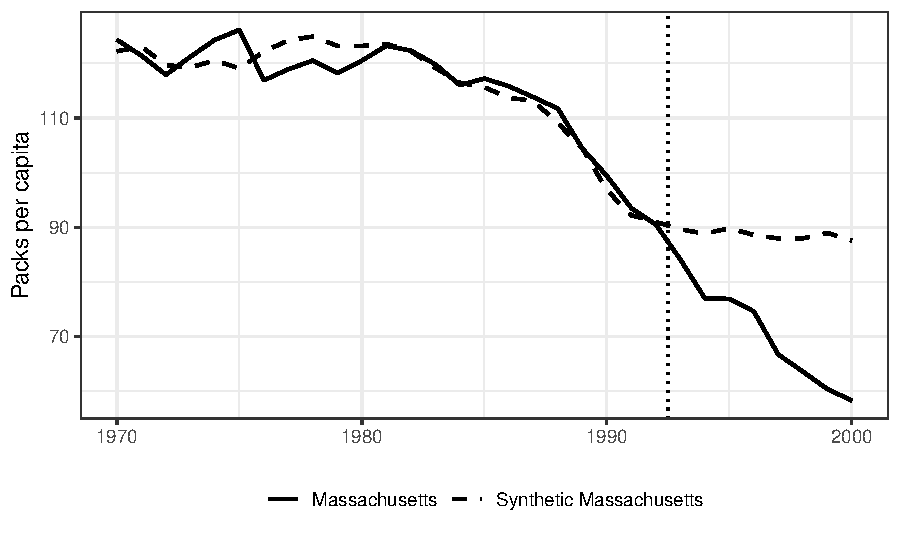
\includegraphics[width=\linewidth]{ma_path.pdf}
\caption{Massachusetts and synthetic Massachusetts}\end{subfigure}\hfill
\begin{subfigure}{0.49\textwidth}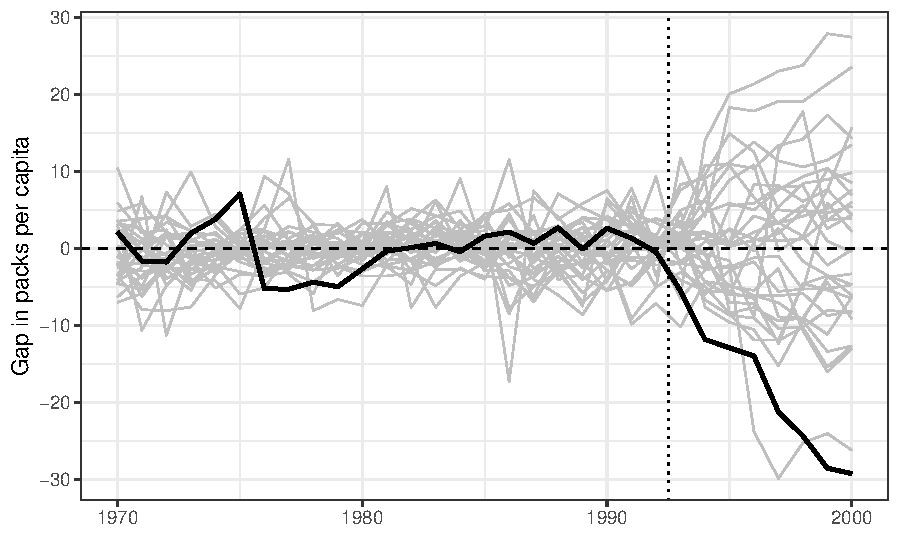
\includegraphics[width=\linewidth]{ma_placebo.pdf}
\caption{Gaps: Massachusetts (black) and placebos (grey)}\end{subfigure}
\caption{Synthetic control estimates for Massachusetts. Panel (b) omits placebos
whose pre-treatment MSPE is more than five times that of Massachusetts.}\label{fig:ma}
\end{figure}

Figure~\ref{fig:ma}(b) compares the Massachusetts gap with the 38 placebo gaps.
Massachusetts' gap is the most negative of any state by the late 1990s, but the
two-sided test is less decisive than for California. Missouri and Oklahoma have
larger post/pre RMSPE ratios than Massachusetts, because their sales rose
relative to their synthetic controls, so the two-sided permutation $p$-value is
$3/39 = 0.077$. Ranking the signed standardised effect instead, no placebo
shows a reduction as large as Massachusetts', giving a one-sided $p$-value of
$1/39 = 0.026$. The one-sided test matches the hypothesis of interest (that the
program reduced sales), but it was chosen after seeing that the two-sided test
was weakened by placebo increases, so I treat 0.077 as the headline number.

\subsection{Comparison with DiD and synthetic DiD}
Table~\ref{tab:main} reports average post-treatment effects from all
estimators. For Massachusetts they lie between $-15.7$ and $-19.3$ packs, a
narrow range. The agreement is less tight for California, where TWFE DiD
($-27.4$) is about 50\% larger than the synthetic control estimate ($-17.8$):
California's sales were already falling faster than the donor average before
1988, and equal donor weights attribute part of that pre-existing decline to
Proposition~99. For Massachusetts the close agreement is partly a coincidence,
as the event study below shows.

\begin{table}[H]\centering\small
\caption{Average effect on per-capita cigarette sales (packs) in the post-treatment period.}\label{tab:main}
\begin{tabular}{lcc}
\toprule
 & California (1989) & Massachusetts (1993) \\
\midrule
Two-way FE DiD & -27.4 & -19.3 \\
 & (2.8) & (2.5) \\
 & [0.128] & [0.179] \\
\addlinespace
Synthetic control (ADH predictors) & -17.8 & -18.5 \\
 &  &  \\
 & [0.026] & [0.077] \\
\addlinespace
Synthetic control (outcomes only) & -19.6 & -15.7 \\
 & (11.9) & (11.1) \\
\addlinespace
Synthetic DiD & -15.2 & -16.9 \\
 & (9.9) & (10.8) \\
\bottomrule
\end{tabular}

\par\smallskip\footnotesize Parentheses: cluster-robust (TWFE) or placebo (synthdid)
standard errors. Brackets: placebo-in-space permutation $p$-values. TWFE
$p$-values rank $|\hat\tau|$ across the 39 units; the synthetic control $p$-value
ranks the post/pre RMSPE ratio. Rows 3 and 4 are from the \texttt{synthdid}
package.
\end{table}

The table also shows how much the inferential method matters. TWFE
cluster-robust standard errors of 2.5--2.8 packs would make every estimate look
highly significant, but they are invalid with one treated cluster. The
permutation $p$-values for TWFE are 0.13 (California) and 0.18
(Massachusetts): several donor states saw sales changes of similar size relative
to the donor average. The synthdid placebo standard errors are 10--12 packs;
the 95\% interval for Massachusetts' synthetic DiD estimate is roughly
$[-38, 4]$ packs. Synthetic control, which fits each state's own pre-period,
is the only method under which Massachusetts stands out clearly from the
placebos.

The event study (Figure~\ref{fig:es} in the appendix) shows why parallel
trends with equal donor weights is not credible for Massachusetts. Relative to
1992, the pre-treatment coefficients are far from zero and move in both
directions: about $+17$ in 1970, between $-12$ and $-5$ in 1976--1980, and $+7$
to $+11$ in 1985--1990, falling to zero by 1992. Massachusetts was already
losing sales faster than the average donor in the late 1980s, which on its own
would make a DiD estimate too negative; the TWFE estimate averages over all of
these pre-period deviations, and they partly offset each other. The post-1993
coefficients ($-6$ in 1993, about $-24$ by 1998--1999) are therefore hard to
read as effects. Synthetic control handles the problem by choosing donors
whose late-1980s decline matches Massachusetts', which is why its estimate,
rather than the DiD one, is the main result.

\paragraph{Price channel.}
Relative to the donors, Massachusetts' log retail price rose by 0.127 (about
13.5\%) after 1992, and log sales fell by 0.272 (about 24\%). The implied
elasticity is $-2.1$ (Table~\ref{tab:elas}); for California it is $-3.4$.
Estimates of the price elasticity of cigarette demand cluster around $-0.4$
\citep{chaloupka2000}. At that elasticity, a 13.5\% price increase would
reduce sales by roughly 5\%, about a fifth of the observed decline. The rest has
to come from channels other than price: the media campaign and other parts of
the program, purchases moved to lower-tax states (which reduce recorded sales
but not necessarily smoking), or changes in Massachusetts that the comparison
does not capture.

\begin{table}[H]\centering\small
\caption{DiD effects on log sales and log price, and the implied elasticity.}\label{tab:elas}
\begin{tabular}{lcc}
\toprule
 & California & Massachusetts \\
\midrule
DiD on log sales & -0.422 & -0.272 \\
DiD on log price & 0.123 & 0.127 \\
Implied price elasticity & -3.44 & -2.14 \\
\bottomrule
\end{tabular}

\end{table}

\subsection{Robustness}
Table~\ref{tab:rob} reports the robustness checks.

\emph{In-time placebo.} Pretending that the program started in 1988 and using
only data up to 1992, the synthetic control (again mostly Connecticut and
Delaware) gives an average gap of $+0.4$ packs over 1988--1992. The method does
not create an effect where there should be none.

\emph{Neighbouring states.} If Massachusetts smokers bought cigarettes in
neighbouring states after the tax increase, those states' recorded sales would
rise and inflate the counterfactual. Dropping Connecticut, New Hampshire, Rhode
Island and Vermont from the donor pool makes the estimate larger, not smaller
($-27.5$ packs on average), so cross-border purchases recorded in the donor
states do not explain the result. It cannot rule out purchases recorded in
Massachusetts' other neighbour, New Hampshire, since New Hampshire has no
weight in any specification.

\emph{Specification and timing.} Using all 23 pre-treatment outcomes as
predictors gives $-15.8$; making 1994, the first full fiscal year of the higher
tax, the first treated year gives $-18.4$.

\emph{Leave-one-out.} Dropping each donor with positive weight in turn gives
average gaps between $-13.7$ (without Delaware or without Utah) and $-26.9$
(without Connecticut); Figure~\ref{fig:loo} in the appendix plots the paths.
The sign never changes, but the size of the effect depends on the composition
of the synthetic control by about a factor of two.

\begin{table}[H]\centering\scriptsize
\caption{Robustness of the Massachusetts synthetic control estimate (packs per capita).}\label{tab:rob}
\resizebox{\textwidth}{!}{\begin{tabular}{llccc}
\toprule
Specification & Donors (weight $\geq 0.05$) & Pre RMSPE & Avg.\ gap & Final gap \\
\midrule
Baseline & CT (0.49), DE (0.29), UT (0.15), RI (0.07) & 3.02 & -18.5 & -29.3 \\
In-time placebo: 1988 (data to 1992) & CT (0.49), DE (0.24), WI (0.14), UT (0.09) & 3.31 & 0.4 & -1.7 \\
Drop CT, NH, RI, VT from donors & DE (0.53), UT (0.31), MN (0.15) & 3.75 & -27.5 & -41.0 \\
All pre-period outcomes as predictors & CT (0.56), DE (0.13), OH (0.11), UT (0.09), RI (0.06) & 2.97 & -15.8 & -24.2 \\
First treated year 1994 & CT (0.52), DE (0.24), UT (0.13), RI (0.11) & 3.09 & -18.4 & -26.7 \\
Drop CT & DE (0.50), UT (0.28), MN (0.22) & 3.78 & -26.9 & -40.0 \\
Drop DE & CT (0.67), IN (0.11), NM (0.09) & 3.49 & -13.7 & -19.9 \\
Drop RI & CT (0.51), DE (0.32), UT (0.15) & 3.11 & -19.8 & -31.2 \\
Drop UT & CT (0.67), IN (0.13), NM (0.10), RI (0.06) & 3.45 & -13.7 & -20.0 \\
\bottomrule
\end{tabular}
}
\par\smallskip\footnotesize Average gap over the post-treatment period; final
gap in 2000 (in 1992 for the in-time placebo).
\end{table}

%======================================================================
\section{Conclusions and limitations}

Massachusetts' 1992 tobacco control initiative was followed by a substantial
fall in per-capita cigarette sales relative to a synthetic control that tracked
the state closely for two decades. The average reduction over 1993--2000 is
about 18 packs per capita (21\%), and the gap widens to about 29 packs by 2000.
In proportional terms this is almost the same effect that \citet{adh2010}
estimate for California, which suggests that the California result was not a
one-off. DiD and synthetic DiD point estimates agree, and the in-time placebo
and leave-one-out checks support the sign of the effect.

The evidence is weaker than the point estimates make it look. The study has
several limitations.

\begin{enumerate}
\item \textbf{One treated unit.} The two-sided permutation $p$-value is 0.077,
synthetic DiD's 95\% interval includes zero, and the leave-one-out estimates
range from $-14$ to $-27$ packs. With a single state, the precision of the
estimate is limited by the number of donors and by how well each one is
fitted.
\item \textbf{The treatment is a bundle.} Question~1 raised the tax and funded
the MTCP at the same time, and Massachusetts raised the tax again, to 76 cents,
in 1996 (visible in the data from fiscal 1998). The estimate is the combined
effect of all three. The price-channel calculation suggests that most of the
decline came from something other than the 1993 price increase, but it cannot
say whether that was the program, the later tax increase or tax avoidance.
\item \textbf{Sales are not smoking.} The outcome is tax-paid sales.
Cross-border shopping, internet sales and smuggling reduce Massachusetts' recorded
sales without reducing consumption; \citet{lovenheim2008} documents that this
casual smuggling responds to tax differences between nearby states. The
neighbour test rules out the case in which those purchases inflate the donors'
sales, but not purchases from New Hampshire or from untaxed sources.
\item \textbf{Contaminated donors.} Several donors raised their own taxes after
1992 (Rhode Island from 37 to 71 cents, Connecticut from 40 to 50 cents, Utah by
25 cents in 1999), and many states began tobacco control activities after the
1998 Master Settlement Agreement. If anything, this lowers the counterfactual
and biases the estimated effect toward zero in the last years of the sample.
\item \textbf{Measurement.} The O\&W series is by fiscal year and the
covariates by calendar year, and the covariates used here are current releases
rather than the vintages used by \citet{adh2010}. The replication shows that
these differences matter little for California.
\end{enumerate}

Natural extensions are individual-level outcomes (e.g.\ smoking prevalence
from the CPS Tobacco Use Supplement or BRFSS) to separate smoking from sales,
data on cross-border sales to quantify avoidance, and the augmented synthetic
control estimator of \citet{benmichael2021}, which corrects for imperfect
pre-treatment fit such as Massachusetts' 1975 spike.

%======================================================================
\begin{thebibliography}{99}

\bibitem[Abadie et~al.(2010)]{adh2010}
Abadie, A., Diamond, A., and Hainmueller, J. (2010).
Synthetic control methods for comparative case studies: Estimating the effect
of California's tobacco control program.
\emph{Journal of the American Statistical Association}, 105(490):493--505.

\bibitem[Abadie and Gardeazabal(2003)]{abadie2003}
Abadie, A. and Gardeazabal, J. (2003).
The economic costs of conflict: A case study of the Basque Country.
\emph{American Economic Review}, 93(1):113--132.

\bibitem[Arkhangelsky et~al.(2021)]{arkhangelsky2021}
Arkhangelsky, D., Athey, S., Hirshberg, D.~A., Imbens, G.~W., and Wager, S. (2021).
Synthetic difference-in-differences.
\emph{American Economic Review}, 111(12):4088--4118.

\bibitem[Ben-Michael et~al.(2021)]{benmichael2021}
Ben-Michael, E., Feller, A., and Rothstein, J. (2021).
The augmented synthetic control method.
\emph{Journal of the American Statistical Association}, 116(536):1789--1803.

\bibitem[Biener et~al.(2000)]{biener2000}
Biener, L., Harris, J.~E., and Hamilton, W. (2000).
Impact of the Massachusetts tobacco control programme: Population based trend
analysis. \emph{BMJ}, 321(7257):351--354.

\bibitem[Chaloupka and Warner(2000)]{chaloupka2000}
Chaloupka, F.~J. and Warner, K.~E. (2000).
The economics of smoking. In Culyer, A.~J. and Newhouse, J.~P., editors,
\emph{Handbook of Health Economics}, volume~1B, pages 1539--1627. Elsevier.

\bibitem[Conley and Taber(2011)]{conley2011}
Conley, T.~G. and Taber, C.~R. (2011).
Inference with ``difference in differences'' with a small number of policy
changes. \emph{Review of Economics and Statistics}, 93(1):113--125.

\bibitem[Harris et~al.(1996)]{harris1996}
Harris, J.~E., Connolly, G.~N., Brooks, D., and Davis, B. (1996).
Cigarette smoking before and after an excise tax increase and an antismoking
campaign---Massachusetts, 1990--1996.
\emph{Morbidity and Mortality Weekly Report}, 45(44):966--970.

\bibitem[Lovenheim(2008)]{lovenheim2008}
Lovenheim, M.~F. (2008).
How far to the border? The extent and impact of cross-border casual cigarette
smuggling. \emph{National Tax Journal}, 61(1):7--33.

\bibitem[Orzechowski and Walker(2019)]{orzechowski2019}
Orzechowski and Walker (2019).
\emph{The Tax Burden on Tobacco, 1970--2019}. Distributed by the CDC STATE
System, dataset \texttt{7nwe-3aj9}, \url{https://data.cdc.gov}.

\end{thebibliography}

%======================================================================
\clearpage
\appendix
\section{Additional figures}

\begin{figure}[H]\centering
\begin{subfigure}{0.49\textwidth}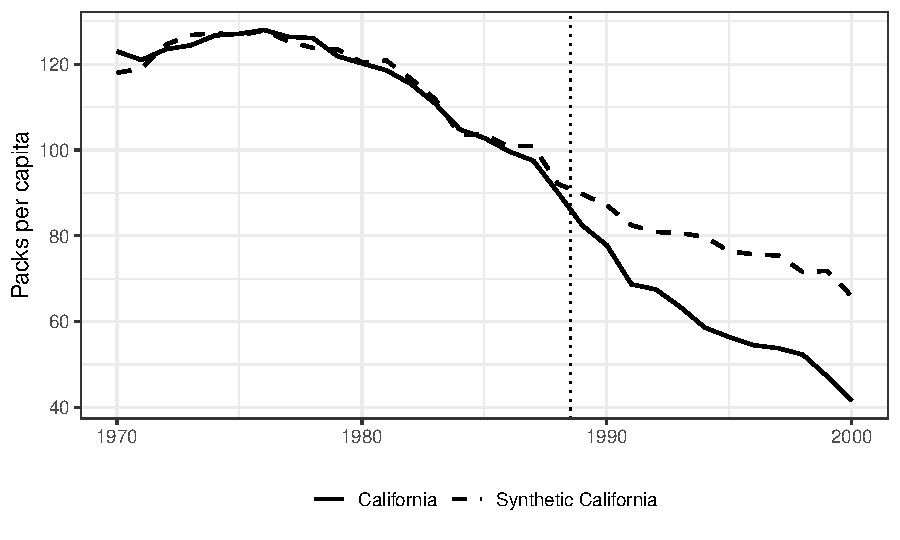
\includegraphics[width=\linewidth]{ca_path.pdf}
\caption{California and synthetic California}\end{subfigure}\hfill
\begin{subfigure}{0.49\textwidth}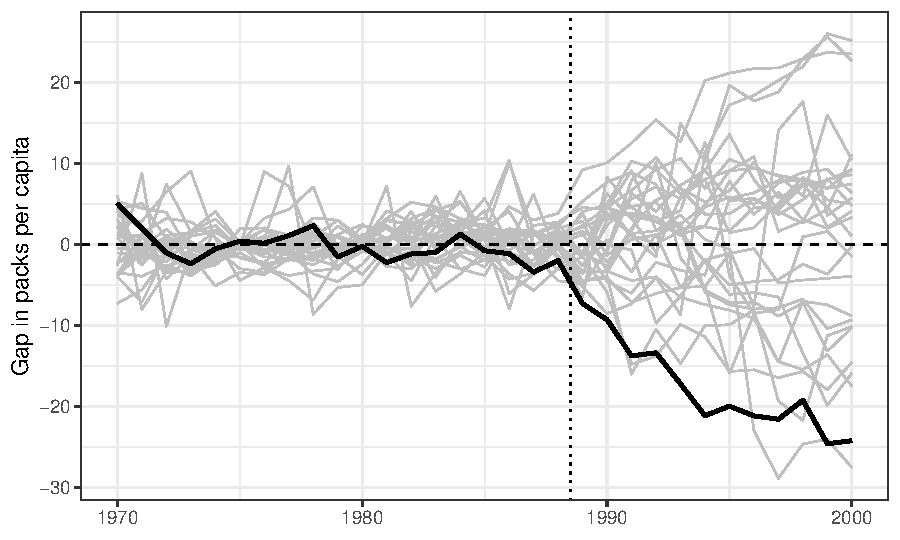
\includegraphics[width=\linewidth]{ca_placebo.pdf}
\caption{Gaps: California (black) and placebos (grey)}\end{subfigure}
\caption{Replication of \citet{adh2010}, Figures 2 and 5.}\label{fig:ca}
\end{figure}

\begin{figure}[H]\centering
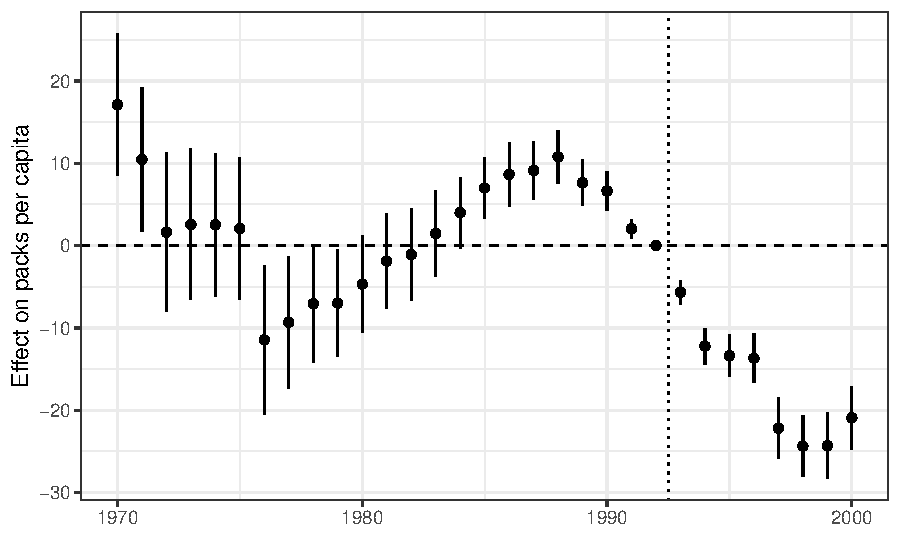
\includegraphics[width=0.7\textwidth]{ma_event_study.pdf}
\caption{TWFE event study for Massachusetts, reference year 1992, with 95\%
cluster-robust intervals (which understate uncertainty with one treated state).}\label{fig:es}
\end{figure}

\begin{figure}[H]\centering
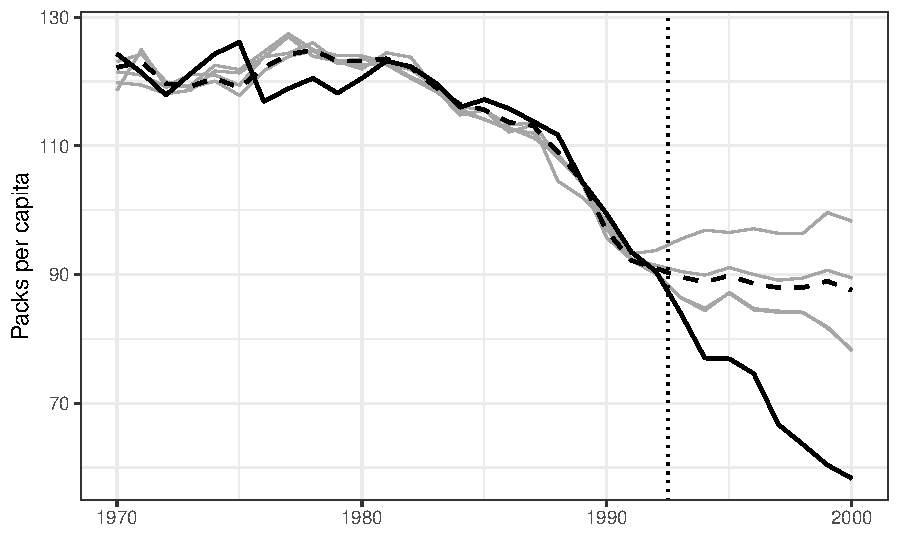
\includegraphics[width=0.7\textwidth]{ma_loo.pdf}
\caption{Leave-one-out: Massachusetts (solid), baseline synthetic control
(dashed) and synthetic controls dropping one positive-weight donor at a time
(grey).}\label{fig:loo}
\end{figure}

\end{document}
